\documentclass[12pt]{article}
\usepackage{scribe}
\usepackage{float}
\newtheorem{assumption}[theorem]{Assumption}
\newcommand{\cC}{\mathcal{C}}
\newcommand{\cX}{\mathcal{X}}
\newcommand{\TV}{\mathrm{TV}}
\newcommand{\Unif}{\mathrm{Unif}}
\newcommand{\Ham}{\mathrm{Ham}}

\lecturetitle{Undetectable Watermarking for Autoregressive Image Models: Does the CGZ Impossibility Transfer?}
\authorname{Raymond Bahng}
\authorname{Isabella Wu}
\authorname{Maureen Zhang}
\lecturedate{May 2026}

\begin{document}
\maketitleblock

\begin{abstract}
[TBD]
\end{abstract}

\section{Introduction}

Christ, Gunn, and Zamir (CGZ) show that undetectable watermarking for
autoregressive language models faces a fundamental limitation: if the
watermark is hidden strongly enough, then a polynomial-time adversary
can remove it by regenerating the output one token at a time. Their
impossibility result is tied to the autoregressive structure itself:
undetectability forces each watermarked next-token distribution to stay
close to the clean one, which enables sequential resampling.

This paper asks whether the same conclusion transfers to autoregressive
image models. At a high level, these models also generate a discrete
sequence autoregressively, so one might expect the CGZ argument to
apply unchanged. But unlike text, the latent token sequence is not the
final object observed by a user. In modern autoregressive image models,
the generated latent sequence must be decoded into pixels through a
learned tokenizer/decoder pipeline. This raises the possibility that a
watermark may be removable in latent space while still being difficult
to remove in image space without degrading perceptual quality.

Our goal is therefore twofold. First, we want a mathematical analog of
the CGZ setting in which we can ask what remains true for
autoregressive image generation. Second, because the real model used in
practice is too complicated to analyze directly, we want an empirical
study that tests whether the relevant image-space phenomena appear in a
concrete open-source model. We use LlamaGen for this purpose because it
is an autoregressive image model with enough implementation access to
modify the sampling loop directly~\cite{llamagen2024}.

The paper has a corresponding two-part structure. The theoretical
analysis introduces a finite-codebook toy model that captures the
latent autoregressive process and a decoder/encoder bottleneck. This
lets us separate what can be proved in latent space from what must be
treated as an image-space assumption. The experimental part implements
CGZ watermarking in LlamaGen and compares removal attacks in both
latent-token and pixel-space settings. Our aim is not to claim a full
theorem about the real model, but to use theory and experiments
together to understand when the CGZ impossibility should be expected to
transfer and when it should not.

\section{Background}
\subsection{CGZ Watermarking and the Section 6.2 Impossibility}

CGZ formalize watermarking for autoregressive language models in terms
of a clean next-token distribution and a keyed watermarked generator
that slightly biases token sampling while preserving fluency. The
detector, given the secret key and a generated sequence, tests whether
the sequence aligns with a hidden keyed pattern more often than chance.
The watermark is designed to satisfy three properties: soundness, so
clean text is rarely flagged; completeness, so watermarked text is
detected with high probability; and undetectability, so an efficient
adversary without the key cannot reliably distinguish watermarked
samples from clean ones~\cite{cgz2024}.

The central negative result in CGZ is the Section~6.2 removal theorem.
For prefix-specifiable autoregressive models, if the watermark is
strongly hidden, then every watermarked conditional next-token law must
remain close to the clean one. An adversary can therefore rebuild the
output token by token from these nearly clean conditionals, producing a
sequence whose distribution is close to the clean model and whose
watermark signal disappears. In short, strong undetectability implies
removability in the autoregressive language-model setting.

This gives the benchmark for our paper. If an autoregressive image model
is viewed only as a discrete autoregressive latent generator, then one
might expect the same impossibility to transfer unchanged. The main
question is what changes once the generated latent sequence is no longer
the final observable object.

\subsection{LlamaGen and VQ-VAE Tokenization}

LlamaGen generates images autoregressively in a discrete latent space
rather than directly in pixels~\cite{llamagen2024}. In the concrete
version we study, a pretrained VQ-VAE tokenizer maps images to a grid
of discrete codebook indices, and the autoregressive model predicts
those indices sequentially. After generation, a decoder maps the latent
grid back to pixels. In our experiments, the relevant latent
representation is a $24\times 24$ grid, i.e., a sequence of $576$
discrete tokens.

We emphasize LlamaGen not because VQ-VAE is the defining feature of all
autoregressive image models, but because it is the accessible model we
can implement on directly. In this system, the decoder/encoder pipeline
creates the main structural asymmetry with the text setting. During
generation, latent tokens are decoded into pixels. But an attacker who
starts from a finished image and tries to return to token space must
apply the encoder as well. Because this round trip is lossy, the
re-encoded latent sequence can change even when the attacked image
remains visually similar.

This is the motivation for separating latent-space and image-space
analysis in the rest of the paper. The latent autoregressive process is
the right level for a CGZ-style theorem, but the decoded image is the
right level for practical evaluation. Since the real encoder/decoder is
too complex to analyze directly, our theoretical section introduces a
toy model that abstracts this bottleneck, and our empirical section
tests how much it matters in LlamaGen itself.

Related work on image watermarking is complementary. Gunn, Zhao, and
Song give a provably undetectable watermark for diffusion models by
embedding signal in the initial latent noise rather than in
autoregressive token choices, using a pseudorandom error-correcting
code construction to select the initial latent~\cite{gunnzhaosong2025,prc2024}.
That result shows that undetectable watermarking is possible in
generative image models, but it does not address the autoregressive
token-by-token removal logic that drives the CGZ impossibility. Other
image watermarking work studies diffusion-based watermarking
schemes~\cite{wen2023,fernandez2023}, removable pixel-space
watermarks~\cite{zhao2024removable}, and watermarking methods tailored
to autoregressive image-token generation~\cite{jovanovic2025}; our
focus is narrower, namely whether the CGZ removability mechanism
transfers to autoregressive image models and how that interacts with a
tokenizer/decoder bottleneck.

\section{Theoretical Analysis}

This section introduces a finite-codebook toy model that captures the
latent autoregressive process and an abstract decoder/encoder
bottleneck. Within this model, we prove a CGZ-style removal theorem in
latent space under a strong latent undetectability assumption, and then
formulate a relaxed image-space notion based on perceptual distortion.
The image-space part is intentionally conditional: it identifies the
extra assumption needed to make removal costly after decoding, rather
than claiming a verified theorem about LlamaGen itself.

\subsection{Finite-Codebook Latent Model}

\begin{definition}[Finite-codebook autoregressive latent model]
Fix a codebook $\cC=\{1,\dots,K\}$, sequence length $L$, and context
length $m$. For each time $t>m$ and context $c\in \cC^m$, let
$A_t(c)\subseteq \cC$ be an admissible set of even cardinality
$M_t(c)\ge 2$. The clean latent generator $P$ samples
$z=(z_1,\dots,z_L)\in \cC^L$ autoregressively by
\[
z_t \sim \Unif(A_t(z_{t-m:t-1})) \qquad \text{for } t=m+1,\dots,L,
\]
with arbitrary initialization on the first $m$ tokens. We write
$c_t(z)=z_{t-m:t-1}$ for the context at time $t$.
\end{definition}

This model retains the autoregressive structure of a latent-token image
generator while remaining simple enough for exact proofs. The admissible
set $A_t(c)$ represents the subset of codebook entries that the clean
model regards as plausible at position $t$ under context $c$.

\begin{definition}[Keyed green sets and watermarking rule]
For each pair $(t,c)$ with $t>m$ and $c\in\cC^m$, the secret key $k$
specifies a subset $G_t^k(c)\subseteq A_t(c)$ of size exactly
$M_t(c)/2$. In the toy model, the family $\{G_t^k(c)\}_{t,c}$ is
sampled independently and uniformly among all half-subsets. The
watermarked latent generator $P_k$ samples
\[
z_t \sim \Unif(G_t^k(z_{t-m:t-1})) \qquad \text{for } t=m+1,\dots,L.
\]
The first $m$ tokens under $P_k$ are sampled from the same
initialization law as under $P$.
The detector score of a sequence $z$ under key $k$ is
\[
S_k(z)=\sum_{t=m+1}^L \mathbf{1}\!\left[z_t\in G_t^k(c_t(z))\right].
\]
The detector outputs $\mathrm{Det}_k(z)=1$ iff $S_k(z)\ge \tau$.
\end{definition}

Intuitively, the key selects a secret green half of the admissible
tokens at each time and context. The watermarked sampler draws only from
this green set, while the detector checks whether the resulting latent
sequence lands in the keyed green set unusually often.

\subsection{Latent-Space Undetectability, Soundness, and Completeness}

\begin{definition}[One-shot latent undetectability]
We say the watermark is one-shot latent-undetectable if, when the secret
key is sampled at random and hidden from the adversary, the distribution
of a single completed latent sample from $P_k$ is identical to that of a
single completed latent sample from $P$.
\end{definition}

\begin{theorem}[One-shot latent undetectability]
In the toy model above, the watermark is one-shot latent-undetectable:
for every measurable set $B\subseteq \cC^L$,
\[
\Prob[k,z\sim P_k]{z\in B}=\Prob[z\sim P]{z\in B}.
\]
\end{theorem}

The proof is a direct induction on prefix length and is deferred to
Appendix~A. The key observation is that, after averaging over the random
key, the watermarked next-token law at each fresh time/context pair
matches the clean uniform law on the admissible set.

This theorem is deliberately weaker than CGZ's full adaptive-oracle
notion. It is an averaged-over-the-key, single-sample statement. It
does not imply indistinguishability for multiple samples generated with
the same key, since repeated use of the same keyed green sets can
introduce detectable correlations. Its role here is mainly to formalize
the simplest latent setting in which one completed sample reveals no
watermark information without the key.

\begin{theorem}[Soundness]
Set
\[
\tau = \frac{L-m}{2} + \sqrt{\frac{(L-m)\log(1/\alpha)}{2}}.
\]
Then for every key $k$,
\[
\Prob[z\sim P]{\mathrm{Det}_k(z)=1} \le \alpha.
\]
\end{theorem}

Appendix~A gives the full martingale proof. Under the clean model, each
indicator $\mathbf{1}[z_t\in G_t^k(c_t(z))]$ has conditional
expectation $1/2$, so Azuma--Hoeffding yields the threshold above.

\begin{theorem}[Completeness]
If $\tau \le L-m$, then for every key $k$,
\[
\Prob[z\sim P_k]{\mathrm{Det}_k(z)=1}=1.
\]
\end{theorem}

This is immediate from the construction: under $P_k$, every token after
the first $m$ positions lies in the keyed green set, so
$S_k(z)=L-m$ deterministically. A complete proof is included in
Appendix~A.

For the soundness threshold above, deterministic completeness holds
provided
\[
\frac{L-m}{2} + \sqrt{\frac{(L-m)\log(1/\alpha)}{2}} \le L-m,
\]
or equivalently,
\[
\alpha \ge e^{-(L-m)/2}.
\]

\subsection{CGZ-Style Removal in Latent Space}

\begin{definition}[Prefix-specifiable watermarking scheme]
Let $P$ be a clean autoregressive generator on $\cC^L$. A keyed
watermarking scheme consists of a family of conditional next-token
distributions $\{P_k(\cdot \mid u)\}_{k,u}$ indexed by a secret key $k$
and prefixes $u\in \cC^{<L}$. The scheme is prefix-specifiable if an
adversary may query the oracle $P_k(\cdot \mid u)$ on any prefix $u$ of
its choice.
\end{definition}

\begin{definition}[Strong latent undetectability]
A prefix-specifiable watermarking scheme is called strongly
latent-undetectable with parameter $\varepsilon$ if for every key $k$,
every prefix $u$, and every time step $t=|u|+1$,
\[
\TV\!\left(P_k(\cdot \mid u),\,P(\cdot \mid u)\right)\le \varepsilon.
\]
Here $P(\cdot\mid u)$ is understood as the clean next-token conditional
law at prefix $u$.
\end{definition}

This fixed-key, every-prefix condition is much stronger than the
averaged-over-the-key, one-shot undetectability proved for the
half-green toy watermark in Theorem~1. In particular, for the
half-green construction itself and any fixed key $k$ and prefix $u$,
\[
\TV\!\left(\Unif(G_t^k(c_t(u))),\,\Unif(A_t(c_t(u)))\right)=\frac{1}{2},
\]
so the strong latent-undetectability parameter is not small. Theorem~4
should therefore be read as a separate CGZ-style statistical lemma
about any prefix-specifiable watermarking scheme whose fixed-key
conditionals remain uniformly close to the clean conditionals, rather
than as a theorem applied directly to the half-green toy construction.

\begin{theorem}[CGZ-style latent removal]
Let $(P_k,\mathrm{Det}_k)$ be a prefix-specifiable watermarking scheme
that is strongly latent-undetectable with parameter $\varepsilon$, and
suppose that
\[
\Prob[z\sim P]{\mathrm{Det}_k(z)=1}\le \alpha
\]
for every key $k$. Consider the adversary $A$ that constructs
$\tilde z=(\tilde z_1,\dots,\tilde z_L)$ sequentially by querying the
watermarked model on its current prefix and sampling
\[
\tilde z_t \sim P_k(\cdot \mid \tilde z_{1:t-1}).
\]
Then for every key $k$,
\[
\TV\!\left(\mathcal{L}(\tilde z),\,P\right)\le \min\{1,L\varepsilon\},
\]
and consequently
\[
\Prob[\tilde z\sim \mathcal{L}(\tilde z)]{\mathrm{Det}_k(\tilde z)=1}
\le \alpha + L\varepsilon.
\]
\end{theorem}

The full proof is deferred to Appendix~B. The argument is the standard
CGZ coupling idea: at each prefix, maximally couple one draw from the
watermarked conditional with one draw from the clean conditional.
Strong latent undetectability bounds the divergence probability at each
step by $\varepsilon$, so a union bound yields total variation at most
$L\varepsilon$ over the full regenerated sequence. The detector bound
then follows by comparing probabilities of the detection event under the
two sequence laws.

\begin{corollary}[Clean regeneration removal]
Suppose the detector satisfies
\[
\Prob[z\sim P]{\mathrm{Det}_k(z)=1}\le \alpha
\]
for every key $k$. If an adversary discards the original latent
sequence and regenerates a fresh sequence $\tilde z\sim P$, then
\[
\Prob[\tilde z\sim P]{\mathrm{Det}_k(\tilde z)=1}\le \alpha.
\]
\end{corollary}

This corollary is the formal statement most directly aligned with our
experimental token-by-token regeneration attack. It does not preserve
the original image; instead, it produces a fresh clean sample from the
same class-conditional latent distribution.

This is a statistical analog of the CGZ token-by-token removal
phenomenon. If every conditional law of the watermarked model is
uniformly close to the clean conditional law, then sequential
regeneration washes out the watermark up to the clean false-positive
rate.

In particular, if the same scheme were also perfectly complete under
this sequential sampling attack, then one would need
\[
L\varepsilon \ge 1-\alpha.
\]
Thus no prefix-specifiable scheme can simultaneously have small clean
false-positive rate, perfect completeness, and uniformly tiny per-step
statistical deviation from the clean model.

The main takeaway of the latent analysis is therefore negative: at the
autoregressive token level, our toy image model behaves like the CGZ
language-model setting. Strong enough latent undetectability still leads
to removability. Any distinction between the image and text settings
must therefore come from how latent changes are mediated by decoding and
re-encoding, not from the autoregressive latent process alone.

\subsection{Decoder Layer and Perceptual Relaxation}

To model images rather than bare latent strings, we compose the latent
model with a decoder
\[
D:\cC^L\to \cX
\]
and an encoder
\[
E:\cX\to \cC^L.
\]
The round trip
\[
T=E\circ D
\]
is the toy analog of the VQ-VAE decode--re-encode path.

\begin{definition}[Perceptual undetectability]
For each key $k$, let
\[
Q=D(P)
\qquad\text{and}\qquad
Q_k=D(P_k)
\]
be the clean and watermarked decoded image distributions. Fix a class
$\mathcal{H}$ of efficiently computable image distinguishers. We say the
watermark is $(\mathcal{H},\delta)$-perceptually undetectable if, for
every key $k$,
\[
\sup_{h\in \mathcal{H}}
\left|
\Prob[x\sim Q]{h(x)=1}-\Prob[x\sim Q_k]{h(x)=1}
\right|
\le \delta.
\]
\end{definition}

\begin{definition}[$r$-robust latent watermark]
Fix a detector $\mathrm{Det}_k$ on latent sequences. We say the
watermark is $r$-robust if for every key $k$, every latent sequence
$z$ in the support of $P_k$ with $\mathrm{Det}_k(z)=1$, and every
sequence $z'$ satisfying $\mathrm{Det}_k(z')=0$, one has
\[
\Ham(z,z')\ge r.
\]
\end{definition}

\begin{assumption}[Decoder distortion lower bound]\label{assump:decoder}
There exists a nondecreasing function
$\psi:\{0,\dots,L\}\to \mathbb{R}_{\ge 0}$ such that for all latent
sequences $z,z'\in \cC^L$,
\[
d_{\mathrm{img}}(D(z),D(z'))\ge \psi(\Ham(z,z')).
\]
\end{assumption}

\begin{assumption}[Triangle inequality for $d_{\mathrm{img}}$]
\label{assump:metric}
The image-space dissimilarity $d_{\mathrm{img}}$ satisfies the triangle
inequality on the family of images considered in the pixel-space attack
analysis.
\end{assumption}

This assumption should be viewed as a strong image-space separation
condition. It says that sufficiently large latent Hamming changes cannot
be hidden by the decoder without causing nontrivial image-space
distortion. We do not verify this assumption for LlamaGen; in the real
model, whether it is approximately true is an empirical question.

\begin{theorem}[Latent-space removal requires image distortion]
Assume the watermark is $r$-robust and Assumption~\ref{assump:decoder}
holds. Let $z$ be a watermarked latent sequence with
$\mathrm{Det}_k(z)=1$, and let $z'$ be any attacked latent sequence
with $\mathrm{Det}_k(z')=0$. Then
\[
d_{\mathrm{img}}(D(z),D(z'))\ge \psi(r).
\]
In particular, any latent-space attack that removes the watermark by
producing a decoded image $D(z')$ must incur distortion at least
$\psi(r)$ relative to $D(z)$.
\end{theorem}

\begin{proof}
Since the watermark is $r$-robust and $\mathrm{Det}_k(z')=0$, we have
\[
\Ham(z,z')\ge r.
\]
Assumption~\ref{assump:decoder} then gives
\[
d_{\mathrm{img}}(D(z),D(z'))\ge \psi(\Ham(z,z'))\ge \psi(r),
\]
using monotonicity of $\psi$.
\end{proof}

The theorem isolates the additional assumption needed to weaken the
practical force of the latent-space CGZ-style removal argument in the
image setting. Unlike text, image models interpose a decoder and, for
pixel-space attacks, an encoder. If the latent changes required to erase
the watermark must cross a nontrivial perceptual threshold after
decoding, then successful latent-space removal is no longer free in
observable image space.

For arbitrary pixel-space attacks, one needs an additional assumption
relating the attacked image to its re-encoded latent representation. For
example, suppose an attacked image $x'$ satisfies
\[
d_{\mathrm{img}}(x',D(E(x'))) \le \eta.
\]
If $z'=E(x')$ removes the watermark, then the previous theorem and the
triangle inequality from Assumption~\ref{assump:metric} imply
\[
d_{\mathrm{img}}(D(z),x')
\ge
d_{\mathrm{img}}(D(z),D(E(x'))) - d_{\mathrm{img}}(x',D(E(x')))
\ge
\psi(r)-\eta.
\]
Thus, under an additional reconstruction-quality assumption, the same
latent robustness condition also implies a lower bound on the perceptual
distortion of pixel-space removal attacks.

\section{Experimental Setup}
\subsection{Watermark and Dataset}

We implement the CGZ green-list watermark directly in LlamaGen's
class-conditional autoregressive sampling loop~\cite{llamagen2024}. At
generation step $t$, the secret key, the position, and the previous
$m=4$ image tokens are hashed with HMAC-SHA256 to choose a green half
$G_t\subset [V]$ of the VQ codebook, where $V=16384$. After applying
temperature scaling and top-$k$ filtering with $k=2000$, the
watermarked sampler zeros out red-token probabilities and samples from
the renormalized green distribution. The first four image tokens are
sampled normally, so the detector scores $L-m=572$ positions in the
$24\times24$ token grid.

For a token sequence $z$, the detector computes
\[
S_k(z)=|\{t\ge m: z_t\in G_t(c_t(z))\}|
\]
and declares a watermark if $S_k(z)\ge \tau$. We use the soundness
threshold from Section~3 with $\alpha=0.01$:
\[
\tau = \frac{L-m}{2}+\sqrt{\frac{(L-m)\log(1/\alpha)}{2}}
=322.3,
\]
where $L-m=572$ scored positions. We generate 1,000 clean and 1,000
watermarked ImageNet-class-conditional images using LlamaGen-L with
classifier-free guidance scale 4.0, temperature 1.0, and top-$k=2000$.
The baseline detector has true positive rate (TPR) 1.000 on watermarked
samples and false positive rate (FPR) 0.000 on clean samples.

\subsection{Evaluation Axes}

The experiments are designed to test the distinction isolated in
Section~3: latent regeneration can remove the watermark, but
image-space attacks may need to trade perceptual fidelity for enough
latent disruption. We therefore report four quantities.

\textbf{Watermark survival} is the fraction of attacked watermarked
images still detected. We also report the mean post-attack detection
score and compare it to the threshold $\tau=322.3$.

\textbf{Image distortion} is measured by LPIPS~\cite{lpips2018} between
each original watermarked image and its attacked counterpart. Lower is
better. For distribution-level shift, we report FID between attacked
images and the original watermarked images.

\textbf{Latent disruption} is the fraction of VQ tokens changed relative
to the original watermarked token sequence. For token regeneration this
is reported as 100\%, but with the caveat that the attack intentionally
creates a fresh sample rather than preserving the original image.

\textbf{Attack access} records whether the attack queries the
autoregressive model. We distinguish this axis from the quality metrics
because latent token regeneration and image-space attacks have different
adversary access models.

\subsection{Attacks}

The attacks intentionally use different access models, summarized in
Table~\ref{tab:attack_access}. Token regeneration tests the latent CGZ
removal mechanism under access to the clean autoregressive sampler,
whereas the VQ-VAE and diffusion attacks test image-space adversaries
that receive the watermarked image and make no LlamaGen queries.

\begin{table}[H]
\centering
\resizebox{\linewidth}{!}{%
\begin{tabular}{lrrrrl}
\toprule
\textbf{Attack} & \textbf{AR queries} & \textbf{Uses AR model} &
\textbf{Uses VQ encoder} & \textbf{Uses diffusion} & \textbf{Image-preserving?} \\
\midrule
Token regeneration & 576 & yes & no & no & no \\
VQ-VAE roundtrip & 0 & no & yes & no & yes \\
Diffusion regeneration & 0 & no & yes & yes & strength-dependent \\
\bottomrule
\end{tabular}
}
\caption{Attack access model for the three removal strategies. AR
queries count calls to the LlamaGen autoregressive sampler per image.}
\label{tab:attack_access}
\end{table}

\textbf{Token regeneration.} Given the ImageNet class label, the
adversary discards the watermarked token sequence and samples a fresh
sequence from the clean LlamaGen model,
\[
\tilde z_t\sim P(\cdot\mid \tilde z_{1:t-1},c).
\]
This is the empirical version of the clean-regeneration corollary in
Section~3. It uses 576 autoregressive next-token queries per image and
does not require the watermark key.

\textbf{VQ-VAE roundtrip.} Given a watermarked image $x$, the adversary
encodes it with the public VQ-VAE encoder, obtains quantized tokens
$\hat z=E(x)$, and decodes them back to pixels. This attack uses no
autoregressive model queries and directly tests whether the tokenizer
roundtrip alone disrupts enough tokens to defeat detection.

\textbf{Diffusion regeneration.} Given a watermarked image $x$, the
adversary uses Stable Diffusion v1.5 in image-to-image mode with the
prompt ``a high quality photo of a \{ImageNet class name\}.'' We set
the img2img scheduler to 30 inference steps, use guidance scale 7.5,
negative prompt ``low quality, blurry, distorted,'' and sweep strengths
$s\in\{0.01,0.02,0.04,0.08\}$. The regenerated image is then encoded
with the same VQ-VAE tokenizer before detection.

\section{Results}

\subsection{Common Comparison}

Table~\ref{tab:common_results} compares the three attacks on the common
metrics. For diffusion regeneration we use strength $s=0.04$ as the
representative operating point, because it is the weakest tested
strength that completely removes the watermark.

\begin{table}[H]
\centering
\resizebox{\linewidth}{!}{%
\begin{tabular}{lrrrrr}
\toprule
\textbf{Attack} & \textbf{Survival} & \textbf{LPIPS} & \textbf{FID} &
\textbf{Mean score} & \textbf{Tokens changed} \\
\midrule
Token regeneration & 0.0\% & 0.673 & 43.17 & 286.1 & 100.0\% \\
VQ-VAE roundtrip & 90.8\% & 0.026 & 2.91 & 398.0 & 22.3\% \\
Diffusion regeneration ($s=0.04$) & 0.0\% & 0.048 & 8.06 & 287.2 & 75.2\% \\
\bottomrule
\end{tabular}
}
\caption{Common metrics for the representative setting of each attack.
Diffusion uses strength $s=0.04$; detection uses threshold
$\tau=322.3$.}
\label{tab:common_results}
\end{table}

\begin{figure}[H]
\centering
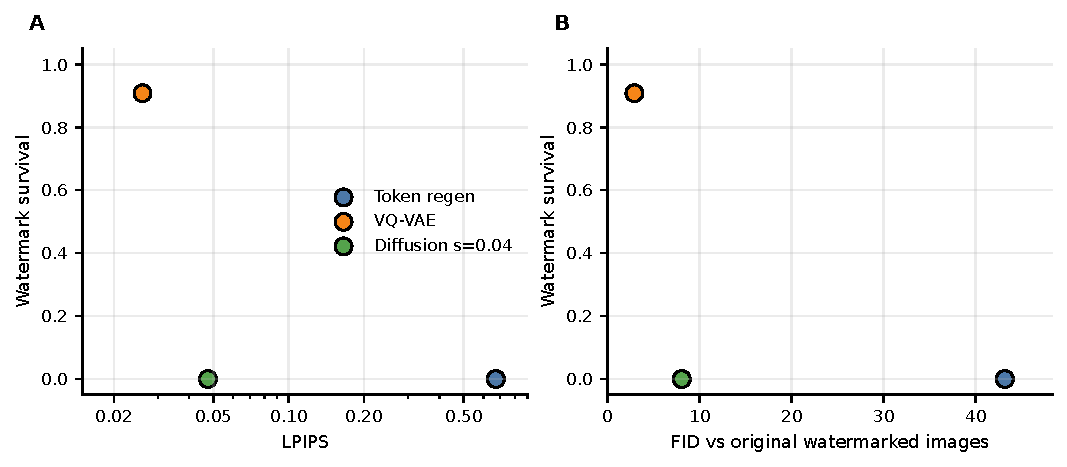
\includegraphics[width=\linewidth]{figures/common_comparison_panel.pdf}
\caption{Common removal-quality comparison. A: watermark survival versus
LPIPS. B: watermark survival versus FID. Token regeneration is a fresh
sample from the clean model; diffusion uses strength $s=0.04$.}
\label{fig:common_quality_tradeoff}
\end{figure}

Wilson 95\% confidence intervals for the survival rates are tight at
this sample size: 0.0--0.38\% for token regeneration, 88.8--92.4\% for
VQ-VAE roundtrip, and 0.0--0.38\% for diffusion at $s=0.04$.

\subsection{Detector Score and Latent Disruption}

\begin{figure}[H]
\centering
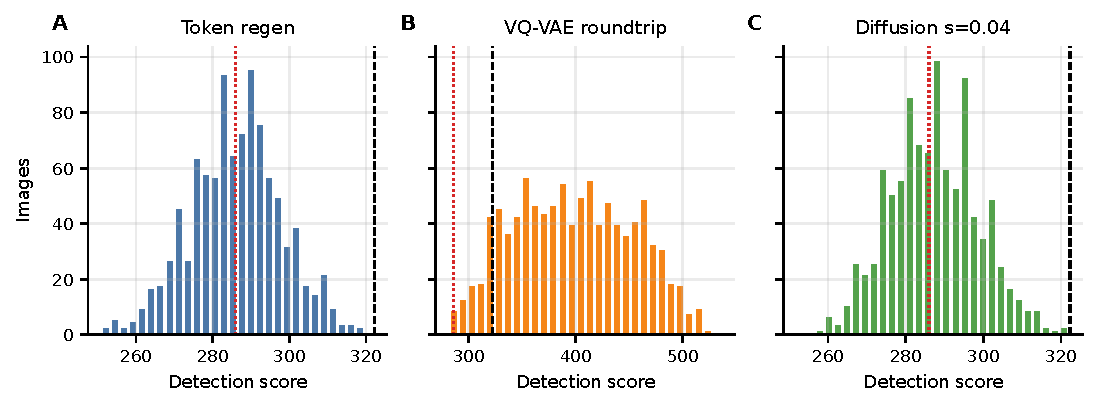
\includegraphics[width=\linewidth]{figures/post_attack_detection_scores.pdf}
\caption{Post-attack detector scores for the representative settings.
A: token regeneration. B: VQ-VAE roundtrip. C: diffusion regeneration at
$s=0.04$. Dashed black lines mark the detection threshold
$\tau=322.3$; dotted red lines mark the clean mean score.}
\label{fig:post_attack_scores}
\end{figure}

\begin{figure}[H]
\centering
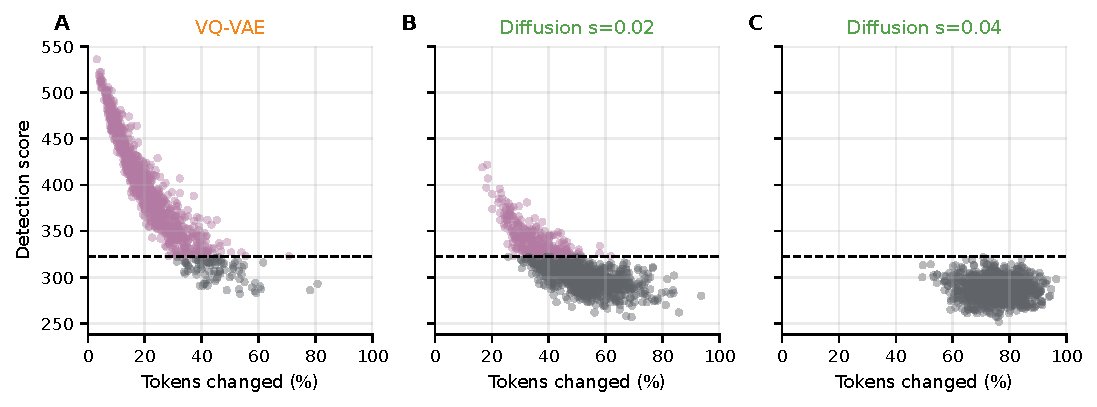
\includegraphics[width=\linewidth]{figures/latent_disruption_vs_detection.pdf}
\caption{Per-image latent disruption versus detector score. A: VQ-VAE
roundtrip. B: diffusion regeneration at $s=0.02$. C: diffusion
regeneration at $s=0.04$. Gray points are removed; purple points are
still detected.}
\label{fig:latent_disruption}
\end{figure}

Token regeneration and diffusion at $s=0.04$ push the score
distribution below threshold, while the VQ-VAE roundtrip usually remains
above threshold. The latent-disruption view explains the separation:
VQ-VAE changes 22.3\% of tokens on average and leaves most watermarks
detected; diffusion at $s=0.02$ changes 47.6\% of tokens on average but
still leaves 27.3\% of watermarks detected; diffusion at $s=0.04$
changes 75.2\% of tokens on average and removes all watermarks.

\subsection{Attack-Specific Observations}

Token regeneration removes the watermark from every tested image and
drives the mean score to 286.1, essentially the clean random-chance
value. Its LPIPS value, 0.673, should not be read as image corruption:
the attack outputs an independent class-conditional sample rather than
an edited version of the original image.

The VQ-VAE roundtrip has low distortion, LPIPS 0.026 and FID 2.91, but
removes only 9.2\% of watermarks. This is the clearest test of the
tokenizer bottleneck: the roundtrip is image-preserving and uses zero
LlamaGen queries, but it usually does not perturb enough tokens to
cross the detector threshold.

Diffusion regeneration is strength-dependent. At $s=0.01$ and
$s=0.02$, survival is still 27.3\%, with LPIPS 0.029 and FID 5.26. At
$s=0.04$, survival falls to 0.0\%, while LPIPS increases to 0.048 and
FID to 8.06. At $s=0.08$, survival remains near zero but LPIPS rises to
0.099 and FID to 22.42.

\section{Discussion}

\section{Conclusion}

\clearpage
\appendix

\section{Proofs for Basic Latent-Space Properties}

\begin{proof}[Proof of Theorem 1]
We prove by induction on time that for every prefix
$u=(u_1,\dots,u_t)$ with $t\ge m$,
\[
\Prob[k,z\sim P_k]{z_{1:t}=u}=\Prob[z\sim P]{z_{1:t}=u}.
\]
The base case $t=m$ is immediate because the initialization law is the
same under $P$ and $P_k$. Assume the claim holds for length
$t-1\ge m$. Fix a prefix $u_{1:t}$. If
$\Prob[z\sim P]{z_{1:t-1}=u_{1:t-1}}=0$, then both the clean and
watermarked probabilities of $u_{1:t}$ are zero, so the claim is
immediate. Otherwise,
\[
\Prob[k,z\sim P_k]{z_{1:t}=u}
=
\Prob[k,z\sim P_k]{z_{1:t-1}=u_{1:t-1}}
\Prob[k,z\sim P_k]{z_t=u_t \mid z_{1:t-1}=u_{1:t-1}}.
\]
Let $c=u_{t-m:t-1}$. Conditional on the event
$z_{1:t-1}=u_{1:t-1}$, the set $G_t^k(c)$ remains independent of the
prefix event, since that event depends only on the initialization law
and on green sets indexed by earlier time steps. Hence $G_t^k(c)$ is
still a uniformly random half-subset of $A_t(c)$.

If $u_t\notin A_t(c)$, then both the clean and watermarked conditional
probabilities are zero. If $u_t\in A_t(c)$, then
\[
\Prob[k,z\sim P_k]{z_t=u_t \mid z_{1:t-1}=u_{1:t-1}}
=
\Prob[k]{u_t\in G_t^k(c)}\cdot \frac{2}{M_t(c)}
=
\frac{1}{2}\cdot \frac{2}{M_t(c)}
=
\frac{1}{M_t(c)}.
\]
This is exactly the clean conditional probability
\[
\Prob[z\sim P]{z_t=u_t\mid z_{1:t-1}=u_{1:t-1}}.
\]
Multiplying by the inductive hypothesis yields equality for prefixes of
length $t$. Taking $t=L$ proves the theorem.
\end{proof}

\begin{proof}[Proof of Theorem 2]
Fix a key $k$. For $t=m+1,\dots,L$, define
\[
X_t = \mathbf{1}[z_t\in G_t^k(c_t(z))].
\]
Conditioned on the past $z_{1:t-1}$, the next token $z_t$ is uniform on
$A_t(c_t(z))$, and $G_t^k(c_t(z))$ contains exactly half of that set.
Hence
\[
\mathbb{E}[X_t \mid z_{1:t-1}] = \frac{1}{2}.
\]
Therefore the process
\[
M_r=\sum_{t=m+1}^{m+r}\left(X_t-\frac{1}{2}\right),
\qquad r=1,\dots,L-m,
\]
is a martingale with increments bounded in $[-1/2,1/2]$. By
Azuma--Hoeffding,
\[
\Pr\!\left[M_{L-m}\ge s\right] \le
\exp\!\left(-\frac{2s^2}{L-m}\right).
\]
Taking
\[
s=\sqrt{\frac{(L-m)\log(1/\alpha)}{2}}
\]
gives
\[
\Pr\!\left[S_k(z)\ge \frac{L-m}{2}+s\right]\le \alpha,
\]
which is exactly the claimed soundness bound.
\end{proof}

\begin{proof}[Proof of Theorem 3]
Under $P_k$, every sampled token satisfies
$z_t\in G_t^k(c_t(z))$ by construction. Therefore $X_t=1$ for every
$t=m+1,\dots,L$, so
\[
S_k(z)=L-m
\]
deterministically. Hence any threshold $\tau\le L-m$ is always exceeded.
\end{proof}

\section{Proof of the CGZ-Style Latent Removal Theorem}

\begin{proof}[Proof of Theorem 4]
We construct a coupling between the adversarial sample $\tilde z$ and a
clean sample $z\sim P$. At each step, as long as the two prefixes agree,
say $\tilde z_{1:t-1}=z_{1:t-1}=u$, couple one draw from
$P_k(\cdot\mid u)$ and one draw from $P(\cdot\mid u)$ using a maximal
coupling. Under such a coupling, the probability that the two next
tokens disagree is exactly
\[
\TV\!\left(P_k(\cdot\mid u),P(\cdot\mid u)\right),
\]
which is at most $\varepsilon$ by strong latent undetectability. Once
the two trajectories diverge, couple the remaining tokens arbitrarily.

Thus, at each step, conditioned on no previous divergence, the
probability of first divergence at that step is at most $\varepsilon$.
By a union bound over the $L$ steps,
\[
\Prob{\,\tilde z\neq z\,}\le L\varepsilon.
\]
By the coupling characterization of total variation distance,
\[
\TV\!\left(\mathcal{L}(\tilde z),\,P\right)\le \min\{1,L\varepsilon\}.
\]
Now let
\[
E=\{\mathrm{Det}_k(\cdot)=1\}.
\]
For any event $E$ and any two distributions $\mu,\nu$, one has
\[
|\mu(E)-\nu(E)|\le \TV(\mu,\nu).
\]
Applying this with $\mu=\mathcal{L}(\tilde z)$ and $\nu=P$ yields
\[
\Prob[\tilde z\sim \mathcal{L}(\tilde z)]{\mathrm{Det}_k(\tilde z)=1}
\le
\Prob[z\sim P]{\mathrm{Det}_k(z)=1}
+ \TV\!\left(\mathcal{L}(\tilde z),P\right)
\le \alpha + L\varepsilon.
\]
\end{proof}

\clearpage
\section{Additional Empirical Diagnostics}

\begin{figure}[H]
\centering
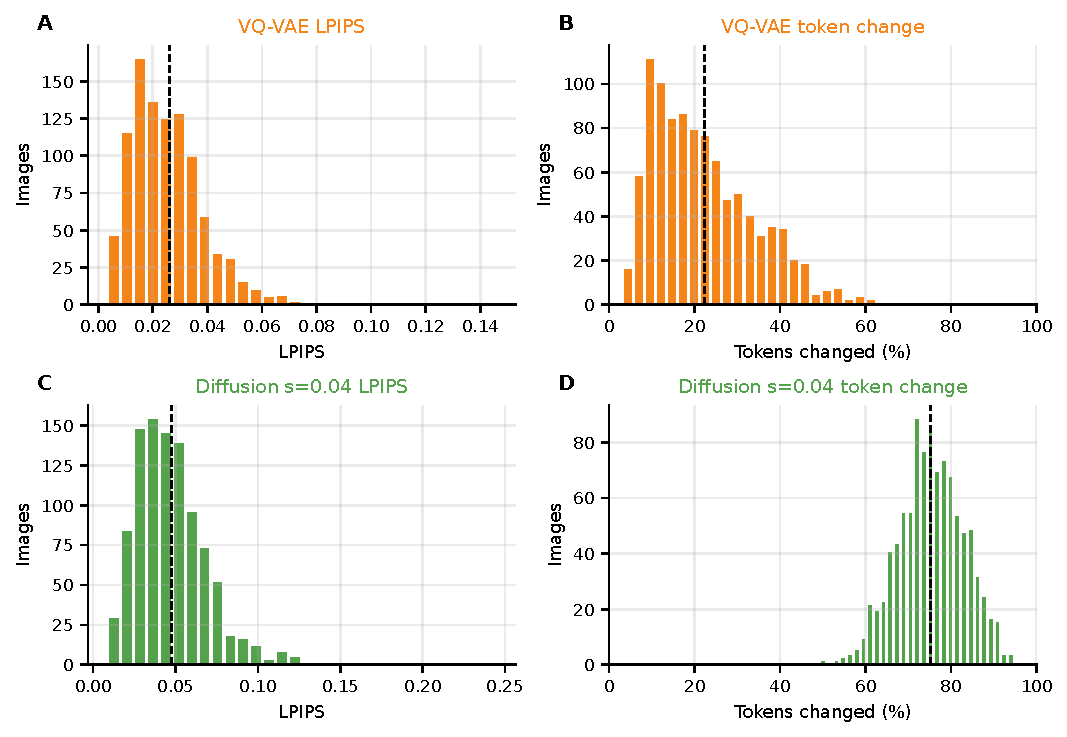
\includegraphics[width=\linewidth]{figures/appendix_quality_diagnostics.pdf}
\caption{Per-image quality and token-change diagnostics. A--B: VQ-VAE
roundtrip LPIPS and token-change distributions. C--D: diffusion
regeneration at $s=0.04$ LPIPS and token-change distributions. Dashed
lines mark means.}
\label{fig:appendix_quality_diagnostics}
\end{figure}

\begin{figure}[H]
\centering
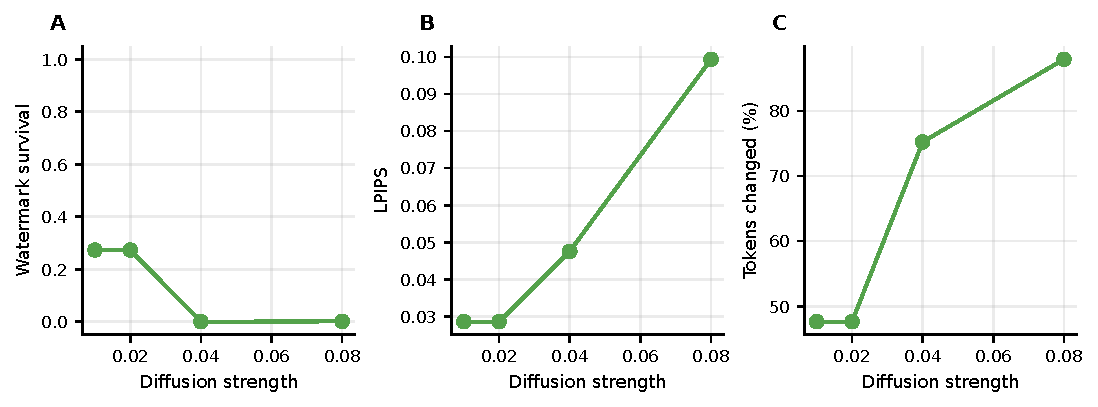
\includegraphics[width=\linewidth]{figures/diffusion_strength_sweep.pdf}
\caption{Diffusion regeneration strength sweep. Increasing strength
reduces watermark survival, but also increases perceptual distortion and
latent token change.}
\label{fig:appendix_diffusion_strength_sweep}
\end{figure}

\bibliographystyle{plainnat}
\bibliography{refs}
\end{document}
